\documentclass[tikz,border=5mm]{standalone}
\usepackage{tikz}
\usetikzlibrary{shapes.geometric, positioning, arrows.meta}

\tikzset{
    node distance=2cm,
    every node/.style={circle, draw, inner sep=4pt},
    edge/.style={->, thick},
    cut edge/.style={thick, dashed},
    label above/.style={above, midway},
    label below/.style={below, midway}
}

\begin{document}
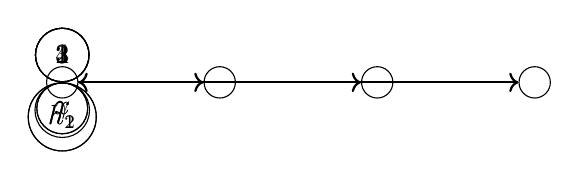
\begin{tikzpicture}
    % Nodes
    \node (A) at (0,0) {};
    \node (B) at (2,0) {};
    \node (C) at (4,0) {};
    \node (D) at (6,0) {};
    
    % Edges
    \draw[edge] (A) -- (B);
    \draw[edge] (B) -- (C);
    \draw[edge] (C) -- (D);
    \draw[edge] (D) -- (A);
    
    % Cut Edge
    \draw[cut edge] (B) -- (C);
    
    % Labels
    \node[label above] at (A) {1};
    \node[label above] at (B) {2};
    \node[label above] at (C) {3};
    \node[label above] at (D) {4};
    
    % Probabilities
    \node[label below] at (A) {$h_1$};
    \node[label below] at (B) {$x$};
    \node[label below] at (C) {$h_2$};
    \node[label below] at (D) {$x$};
    
    % Hybridization Parameter
    \node[label below] at (3,-2) {$\gamma$};
\end{tikzpicture}
\end{document}